\subsection{The Blockchain Trilemma}
The challenge of improving these metrics is often framed as the Blockchain Trilemma \cite{fu2024trilemma}. It suggests that a blockchain architecture can only achieve two out of three desirable properties:
\begin{enumerate}
    \item \textbf{Decentralization:} The network is distributed across many nodes without central control.
    \item \textbf{Security:} The network can resist attacks and manipulation.
    \item \textbf{Scalability:} The network can handle a large volume of transactions at high speed and low cost.
\end{enumerate}

\begin{figure}[H]
    \centering
    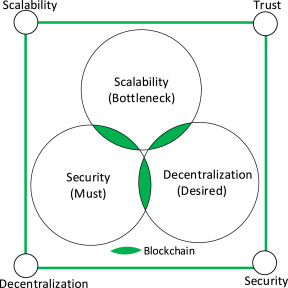
\includegraphics[width=0.90\textwidth]{figures/chapter1/blockchain_trilemma.jpg}
    \caption{Blockchain Trilemma and Quadrilemma.}
    \label{fig:blockchain_trilemma}
\end{figure}

As shown in Figure~\ref{fig:blockchain_trilemma}, the trilemma highlights the trade-offs inherent in blockchain design.
